\documentclass[tikz,border=10pt]{standalone}
\usepackage{amsmath, amssymb, bm}
\usetikzlibrary{positioning, arrows.meta, calc, fit, backgrounds}

\begin{document}
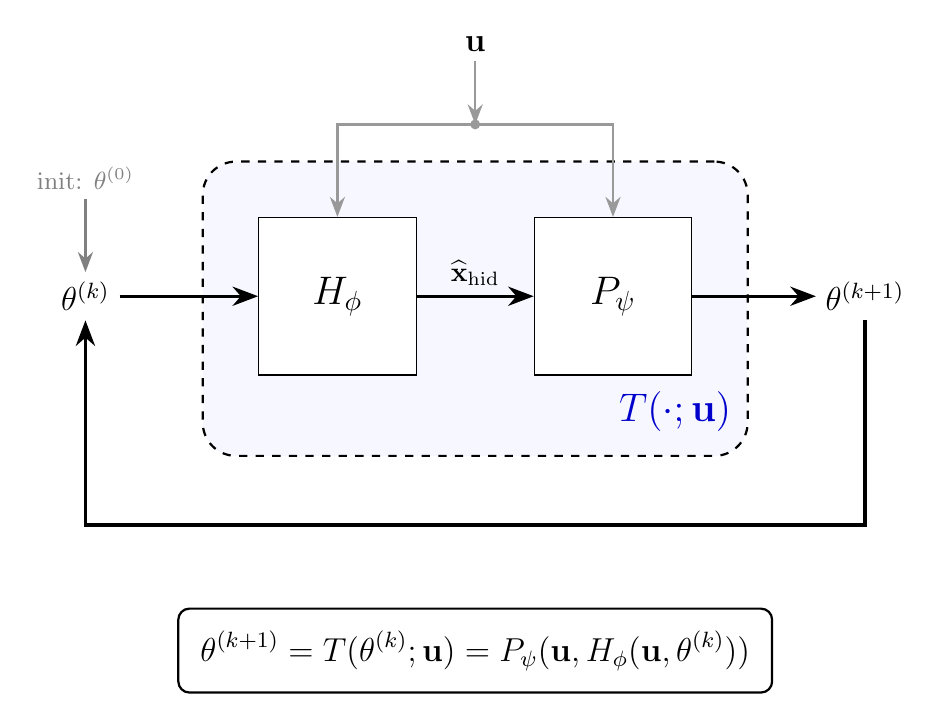
\begin{tikzpicture}[
    >={Stealth[scale=1.1]},
    netbox/.style={draw, rectangle, minimum width=2.0cm, minimum height=2.0cm, align=center, font=\Large, fill=white},
    txt/.style={align=center, font=\large},
    eqbox/.style={draw, rectangle, rounded corners, inner sep=8pt, font=\large, thick},
    uarrow/.style={->, thick, gray!80},
    thetaarrow/.style={->, very thick, black}
]

% 1. Network Blocks (적절하다고 평가하신 내부 간격 유지)
\node[netbox] (H) at (0,0) {$H_\phi$};
\node[netbox] (P) at (3.5,0) {$P_\psi$};

% 2. T Operator Box (내부 여백을 키우고 T 라벨을 위한 공간 확보)
\begin{scope}[on background layer]
    % T 라벨이 P 박스에 가려지지 않도록 하단에 충분한 빈 공간(dummy) 생성
    \node (dummy_bottom) at (3.5, -1.2) {}; 
    \node[draw, rounded corners=12pt, dashed, thick, inner sep=20pt, fit=(H) (P) (dummy_bottom), fill=blue!3] (Tbox) {};
    % 확보된 우측 하단 공간에 T 라벨 배치
    \node[font=\Large\bfseries, text=blue!80!black, anchor=south east, xshift=-0.1cm, yshift=0.2cm] at (Tbox.south east) {$T(\cdot; \mathbf{u})$};
\end{scope}

% 3. Dynamic Variable (외부 화살표 길이를 충분히 늘림)
\node[txt] (theta_in) at (-3.2, 0) {$\theta^{(k)}$};
\node[txt, font=\small, text=gray] (init) at (-3.2, 1.5) {init: $\theta^{(0)}$};
\node[txt] (theta_out) at (6.7, 0) {$\theta^{(k+1)}$};

% 4. Global Parameter (점선 박스와 겹치지 않도록 분기점 높이 상향)
\node[txt] (u_input) at (1.75, 3.2) {$\mathbf{u}$};

\draw[uarrow] (u_input.south) -- ++(0,-0.8) coordinate (u_split);
\draw[uarrow] (u_split) -| (H.north);
\draw[uarrow] (u_split) -| (P.north);
\fill[gray!80] (u_split) circle (1.8pt);

% 5. Main Flow Arrows 
\draw[->, gray, thick] (init) -- (theta_in);
\draw[thetaarrow] (theta_in) -- (H.west);
\draw[thetaarrow] (H.east) -- (P.west) node[midway, above] {$\widehat{\mathbf{x}}_{\mathrm{hid}}$};
\draw[thetaarrow] (P.east) -- (theta_out.west);

% 6. Feedback Loop (커진 T 박스를 완전히 회피하도록 깊게 우회)
\draw[thetaarrow] (theta_out.south) -- ++(0,-2.6) coordinate (loop_right) -- (loop_right -| theta_in.south) coordinate (loop_left) -- (theta_in.south);

% 7. Equation Box below (피드백 루프 아래로 안정적으로 배치)
\node[eqbox] (eq) at (1.75, -4.5) {
    $\displaystyle \theta^{(k+1)} = T(\theta^{(k)}; \mathbf{u}) = P_\psi(\mathbf{u}, H_\phi(\mathbf{u}, \theta^{(k)}))$
};

\end{tikzpicture}
\end{document}